\section{Results}
\label{sec:results}

The campaign ran 59 cells to completion or failure and scored 49, at a measured
cost of \$197.78;\footnote{From the directory-keyed cost report. The aggregate
tool reports \$199.76 because it joins on \code{run\_id}, which two substrates
reuse across sibling replicate directories; we report the former and note the
defect rather than silently choosing.} ten runs produced no score
(Section~\ref{sec:taxonomy}).

\begin{table}[tbp]
\centering
\caption{Per-cell results. $n$ counts \emph{attempts}, so a replicate killed
before writing a deliverable counts against the pass rate; \emph{sc.} counts
those with a frozen-set score. Relative $L_2$ is the median over scored
replicates with a percentile bootstrap interval (10\,000 resamples, seed
\code{20260917}) on the frozen 60-parameter test set, baseline $0.4933$;
``valid'' passes every gate \emph{and} the physical diagnostics of
Section~\ref{sec:validity}, the complement in every cell being a run that passed
every gate while physically invalid. The \Lzero{} row is the pipeline run
directly, so it emits no contract and its interval is the range over three
seeds. \hn{cursor} and \hn{ursa} costs are derived from token counts at a
committed price table, not vendor billing.}
\label{tab:main}
\footnotesize
\setlength{\tabcolsep}{4.5pt}
\begin{tabular}{@{}llrrcrcrr@{}}
\toprule
\textbf{Level} & \textbf{Harness} & $n$ & \textbf{sc.} &
\textbf{pass $k/n$ [Wilson]} &
\textbf{med.} & \textbf{bootstrap CI} &
\textbf{valid} & \textbf{\$} \\
\midrule
\Lzero{} & scripted$^{*}$ & 3 & 3 & n/a & 0.1863 & 0.1774--0.1865 & n/a & 0.00 \\
\midrule
\Ltwo{} & \hn{cursor} & 5 & 5 & 5/5\ \ [0.57, 1.00] & 0.2186 & [0.175, 0.234] & 5/5 & 5.12 \\
\Ltwo{} & \hn{dspy}   & 15 & 10 & 10/15 [0.42, 0.85] & 0.4146 & [0.263, 0.503] & 5/10 & 21.37 \\
\Ltwo{} & \hn{pi}     & 5 & 5 & 5/5\ \ [0.57, 1.00] & 0.1878 & [0.167, 0.211] & 5/5 & 3.94 \\
\Ltwo{} & \hn{ursa}   & 8 & 4 & 4/8\ \ [0.22, 0.79] & 0.6101 & [0.218, 2.494] & 2/4 & 50.71 \\
\midrule
\Lthree{} & \hn{cursor} & 5 & 5 & 5/5\ \ [0.57, 1.00] & \textbf{0.0692} & [0.062, 0.212] & 5/5 & 9.23 \\
\Lthree{} & \hn{dspy}   & 10 & 10 & 10/10 [0.72, 1.00] & 0.1985 & [0.119, 0.229] & 4/10 & 23.46 \\
\Lthree{} & \hn{pi}     & 5 & 5 & 5/5\ \ [0.57, 1.00] & 0.1052 & [0.062, 0.130] & 5/5 & 6.16 \\
\Lthree{} & \hn{ursa}   & 6 & 5 & 5/6\ \ [0.44, 0.97] & 0.2342 & [0.019, 1.084] & 3/5 & 77.79 \\
\bottomrule
\end{tabular}

\vspace{1pt}
{\footnotesize $^{*}$ budget-matched to 450 successful solves, zero LLM calls,
scored by the identical scorer on the identical frozen set.}
\end{table}


\paragraph{Does library access help? (\Ltwo{} vs \Lthree{}).}
\label{sec:l2l3}
It does not: \textbf{from-scratch is better, in every substrate}. Pooled,
\Ltwo{} has median relative $L_2$ $0.2287$ (bootstrap $[0.211, 0.396]$, 24
scored) against \Lthree{}'s $0.1368$ ($[0.077, 0.207]$, 25 scored); pass rates
$24/33$ (Wilson $[0.56, 0.85]$) and $25/26$ ($[0.81, 0.99]$); accuracy per 100
solver calls $10.31$ against $19.55$. The paired differences
(Figure~\ref{fig:levels}) are $-0.149$, $-0.216$, $-0.083$ and $-0.376$.

Our primary test treats harness as a blocking factor and permutes level labels
within it: a stratified rank statistic in the van Elteren family
\citep{vanelteren1960combination}. It gives $z = -4.168$ and permutation
$p = 1/20\,001 \approx 5\times10^{-5}$---zero of 20\,000 within-harness
relabelings reached the observed statistic, so that $p$ is the test's resolution
floor, not a point estimate---and substrate differences cannot inflate it,
because no permutation moves a run between harnesses. Two other tests differ in
power, not direction: the exact sign test on the four paired medians gives
$0/4$, $p = 0.125$, the \emph{smallest attainable} two-sided $p$ at four pairs
whatever the data show; the originally pre-specified median-difference
permutation test gives $\delta = -0.206$, $p = 0.179$, compressing each cell to
one number and then having four. \textbf{The change of primary test was made
after seeing that a unanimous result could not clear the sign test's floor, and
is post-hoc} (Section~\ref{sec:limitations}); all three are printed on every
run.

Two readings survive---library access may genuinely handicap the agent, or the
\Ltwo{} prompt's pointers may anchor agents onto the library's defaults---and
Section~\ref{sec:agentlogic} shows the anchoring is real and measurable.

\begin{figure}[tbp]
\centering
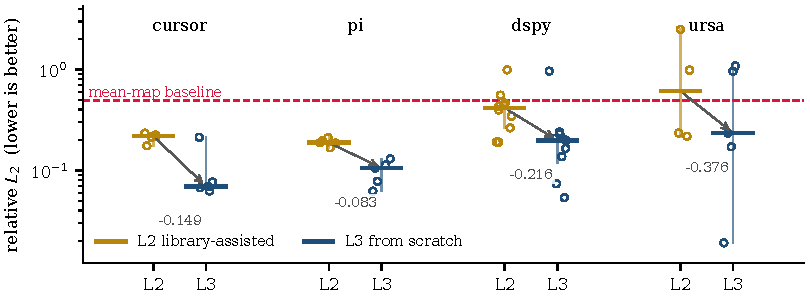
\includegraphics[width=0.68\textwidth]{figures/fig_levels}
\caption{Every scored run, by cell. Circles are replicates, the heavy bar the
cell median with its bootstrap interval, the arrow the within-harness
\Ltwo{}$\rightarrow$\Lthree{} contrast with its median difference. From-scratch
is better in all four substrates, and the two substrates with the widest spread
are the two producing runs worse than the mean-map baseline.}
\label{fig:levels}
\end{figure}

\paragraph{Does the harness matter, with the model held fixed?}
\label{sec:harness-effect}
Yes, and more than the access level does. With \emph{one model} across all eight
cells the per-cell medians span $0.0692$ to $0.6101$, a factor of $8.8$, against
the $1.7\times$ pooled level effect, ordering harnesses \hn{cursor}, \hn{pi},
\hn{dspy}, \hn{ursa} at \Lthree{} and the same but for a \hn{pi}/\hn{cursor}
swap at \Ltwo{}. The spread is not only in the median: \hn{cursor} and \hn{pi}
produced 20 scored runs with \emph{zero} physically invalid artifacts and a
worst case of $0.234$, while \hn{dspy} and \hn{ursa} account for all 15 invalid
artifacts and every run worse than the mean-map baseline. This is the comparison
usually confounded, and the empirical version of a claim recently argued on
other grounds---that the harness, not the model it wraps, is often the binding
constraint \citep{zhang2026harness}.

\paragraph{Against the non-agentic baseline.}
\label{sec:vs-baseline}
The pre-written pipeline, run at \Lzero{} with seeded heuristic decisions and
\emph{no LLM calls at all}, scores mean relative $L_2$ $0.1774$, $0.1865$ and
$0.1863$ on three seeds at a budget matched to the agents' 450 successful
solves---about 63\% accuracy, in 83--101 seconds, for \$0.00 of model spend; given
five times the data it reaches $0.1666$, so the budget is not what limits it.
Against that line, \textbf{two of eight agent cells beat the zero-LLM baseline}
(\Lthree{}-\hn{cursor}, \Lthree{}-\hn{pi}), one matches it and five are worse;
both that beat it are from-scratch. This constrains the reading of
Section~\ref{sec:l2l3}: the library is \emph{not} simply bad code dragging
\Ltwo{} down, since it outperforms five of the eight agent cells on the same
frozen set. The gap is better explained by what library access does to the
agent's search over methods.

\paragraph{Cost and budget compliance.}
\label{sec:cost}
Cost is dominated by one substrate---\hn{ursa} spent \$128.51 across 14 runs,
65\% of the campaign, against \$44.82 (\hn{dspy}), \$14.36 (\hn{cursor}) and
\$10.10 (\hn{pi})---and it buys nothing legible (Appendix~\ref{app:costfig}):
the two cheapest substrates occupy the two best positions and the most expensive
cell sits below \Lthree{}-\hn{pi} at one-thirteenth the price. Costs are measured where a substrate reports dollars and otherwise derived from
token counts at a committed price table; the \hn{cursor} figure is an estimate
at provider rates, not that vendor's billing. On the 450-solve bound the median cell is
compliant once uncapped validation and test solves are allowed for
($239$--$689$ attempted); the exceptions are in \Ltwo{}-\hn{dspy}, whose worst
runs attempted $1914$ and $1650$---overruns of $+1464$ and $+1200$ against a
bound stated in the prompt.
